% PPGMC/FURG Modelo Latex
% Criado em nov/2016 - Marcus Guimaraes <guimaraesmvf@gmail.com>

% Favor quando alterar esse arquivo informar o que foi alterado com comentario
% Este modelo segue as normas estabelecidas pelo PPGMC/FURG

\documentclass[a4paper,12pt,oneside]{article}
\usepackage{ppgmc}
\usepackage[utf8]{inputenc}
\usepackage[brazil]{babel}
\usepackage{amsmath,amssymb}
\usepackage[document]{ragged2e}
\usepackage{setspace}
\usepackage{graphicx}
\usepackage{chngcntr}
\usepackage{indentfirst}
\usepackage{tocloft}
\counterwithin{figure}{section}
\usepackage{etoolbox}
\usepackage{natbib}


\numberwithin{equation}{section}

\makeatletter
\patchcmd{\@caption}{\csname the#1\endcsname}{\csname fnum@#1\endcsname:}{}{}
\renewcommand*\l@figure{\@dottedtocline{1}{1.5em}{5em}}
\let\l@table\l@figure
\makeatother

\makeatletter
\renewcommand*\l@section{\@dottedtocline{1}{0em}{1.5em}}
\makeatother

\renewcommand{\cfttoctitlefont}{\hspace*{\fill}\Large\bfseries}
\renewcommand{\cftaftertoctitle}{\hspace*{\fill}}
\renewcommand{\cftlottitlefont}{\hspace*{\fill}\Large\bfseries\MakeUppercase}
\renewcommand{\cftafterlottitle}{\hspace*{\fill}}
\renewcommand{\cftloftitlefont}{\hspace*{\fill}\Large\bfseries\MakeUppercase}
\renewcommand{\cftafterloftitle}{\hspace*{\fill}}


\begin{document}
\onehalfspacing
\pagestyle{myheadings}

\thispagestyle{empty}
\begin{center}

MINISTÉRIO DA EDUCAÇÃO\\
UNIVERSIDADE FEDERAL DO RIO GRANDE\\
PROGRAMA DE PÓS-GRADUAÇÃO EM MODELAGEM COMPUTACIONAL\\
\vspace*{2.5cm}

%--------------------------------------------------------------------------------------------
% TITULO DO TRABALHO
\vspace{3cm}
\begin{large}
\textbf{\uppercase{
	Título da tese ou dissertação
}}
\end{large}
\vspace*{2cm}\\por\vspace*{2cm}

% NOME DO CANDIDATO
Nome do candidato

\vspace*{2.5cm}
Dissertação para obtenção do Título de\\
Mestre em Modelagem Computacional

% DATA
\vspace{6cm}Rio Grande, mes, ano

\end{center}



%--------------------------------------------------------------------------------------------
% FOLHA DE ROSTO
\newpage
\thispagestyle{empty}


Incluir nesta página a folha de rosto assinada pelos membros da banca. Pode ser utilizado uma\\
fotocópia (xerox) colorida da folha de rosto.


%--------------------------------------------------------------------------------------------
% DEDICATORIA
\newpage
\thispagestyle{empty}
\begin{flushright}\vspace*{5cm}

Dedicatória, opcional feita pelo autor em formato livre,\\
Somente na versão final, após aprovada a dissertação ou tese\\

\end{flushright}


%--------------------------------------------------------------------------------------------
% AGRADECIMENTOS
\newpage
\thispagestyle{empty}
\justify

\begin{center}
\Large{\textbf{AGRADECIMENTOS}}\vspace*{1cm}
\end{center}

Somente na versão final\\


Obrigatório no caso de bolsista para a agência de fomento que financiou a bolsa (CAPES,\\
CNPq, FAPERGS) e a Universidade Federal do Rio Grande (FURG).\\


Opcional para os demais, onde o autor faz agradecimentos dirigidos a pessoas ou\\
instituições que contribuíram de maneira relevante à elaboração do trabalho.\\



%--------------------------------------------------------------------------------------------
% RESUMO
\newpage
\thispagestyle{empty}
\begin{center}
\Large{\textbf{RESUMO}}\vspace*{1cm}
\end{center}

O resumo deve ser escrito em um único parágrafo e não deve conter citações de autores,
fórmulas, abreviaturas, símbolos ou equações. Este deve consistir em um texto claro e objetivo
ressaltando a finalidade, metodologia, resultados e conclusões do trabalho. O resumo, incluindo as
palavras chaves, não pode ultrapassar 1 página de texto. 

\vspace*{1cm}
\textbf{Palavras-chaves:} de 3 a 5 palavras (ou expressões) chaves


%--------------------------------------------------------------------------------------------
% ABSTRACT
\newpage
\thispagestyle{empty}

\begin{center}
\Large{\textbf{ABSTRACT}}\vspace*{1cm}
\end{center}

Mesmas características de formatação do resumo, em língua inglesa, mas não sendo
necessariamente a sua tradução literal. Deve preservar o conteúdo do resumo, adaptando-o às
peculiaridades da língua inglesa.

\vspace*{1cm}
\textbf{Palavras-chaves:} 3 to 5 keywords



%--------------------------------------------------------------------------------------------
% ÍNDICE
\newpage
\thispagestyle{empty}
\vspace*{-33pt}
\renewcommand\contentsname{\centering\Large ÍNDICE}
\tableofcontents



%--------------------------------------------------------------------------------------------
% LISTA DE FIGURAS
\newpage
\thispagestyle{empty}
\vspace*{-33pt}
\listoffigures



%--------------------------------------------------------------------------------------------
% LISTA DE TABELAS
\newpage
\thispagestyle{empty}
\vspace*{-33pt}
\listoftables

%--------------------------------------------------------------------------------------------
% LISTA DE SÍMBOLOS
\newpage
\thispagestyle{empty}
\begin{center}
	\textbf{\Large{LISTA DE SÍMBOLOS}}
\end{center}


\begin{changemargin}{1.5cm}{1.5cm} 
	\begin{tabular}{ll}
		$\alpha$ 	&	Descrição do símbolo\\
		$\beta$ 	&	Descrição do outro símbolo\\
	\end{tabular}
\end{changemargin}

\textbf{Símbolos gregos}
\begin{changemargin}{1.5cm}{1.5cm} 
	\begin{tabular}{ll}
		$\rho$ 	&	massa específica [$kg/m^{3}$]\\
		
	\end{tabular}
\end{changemargin}

\textbf{Sub índices}
\begin{changemargin}{1.5cm}{1.5cm} 
	\begin{tabular}{ll}
		f 	&	fluido\\
		
	\end{tabular}
\end{changemargin}



%--------------------------------------------------------------------------------------------
% LISTA DE ABREVIATURAS
\newpage
\thispagestyle{empty}
\begin{center}
	\textbf{\Large{LISTA DE ABREVIATURAS}}
\end{center}


\begin{changemargin}{1.5cm}{1.5cm} 
	\begin{tabular}{ll}
		ABNT 	&	Associação Brasileira de Normas Técnicas\\

	\end{tabular}
\end{changemargin}





%--------------------------------------------------------------------------------------------
% INICIO DAS SEÇÕES DO TRABALHO

\section{TÍTULO NÍVEL 1}

Introdução da dissertação/tese.

\subsection{Titulo nível 2}

Exemplo de texto em uma subseçao do trabalho.


\subsubsection{Titulo nível 3}

Exemplo de uma subsubseção do trabalho.


\section{INFORMAÇÕES ADICIONAIS}

O texto deve ser escrito de forma impessoal:\\

\noindent- ... fez-se um estudo ...\\
- ... um estudo foi feito ...\\


Deve ser evitado dois títulos (ou sub títulos) que não seja separados por pelo menos um
parágrafo de texto.


\subsection{Formatação das Equações}

As equações devem ser numeradas por capítulo. Estas devem ser centralizadas e a numeração alinhada com a margem esquerda.


Todos os símbolos devem ser descritos no momento de sua primeira aparição no texto e na lista símbolos.


As equações devem ser citadas no texto no formato Eq. \ref{eqExemplo}.


\subsubsection{Exemplo de equação}

A equação da conservação da massa é descrita por

\begin{equation}
\frac{\partial\rho_{f}}{\partial t} + \bigtriangledown \rho_{f} \vec{V}
\label{eqExemplo}
\end{equation}

onde $\rho$ é a massa específica [$kg/m^{3}$], $t$ o tempo [$s$] e  $\vec{V}$ o vetor velocidade [$m/s$].

\subsection{Formatação das figuras}

As figuras devem ser inseridas de forma centralizada e com o título abaixo desta.

A numeração deve ser realizada por capítulos.

Estas devem sempre ser citadas no texto antes de sua aparição. A forma de citação deve ser 


“... é mostrado na Fig. \ref{figExemplo} um exemplo ...” 

quando da citação no meio do texto e na forma:

 “A Figura \ref{figExemplo} mostra ...” quando da citação no início do texto.
 
 
\subsubsection{Exemplo de utilização de figura}

Na Figura \ref{figExemplo} o canal está representado na região cinzenta escuro, enquanto que a região
porosa é representada com cinza claro.


\begin{figure}[h]
\centering
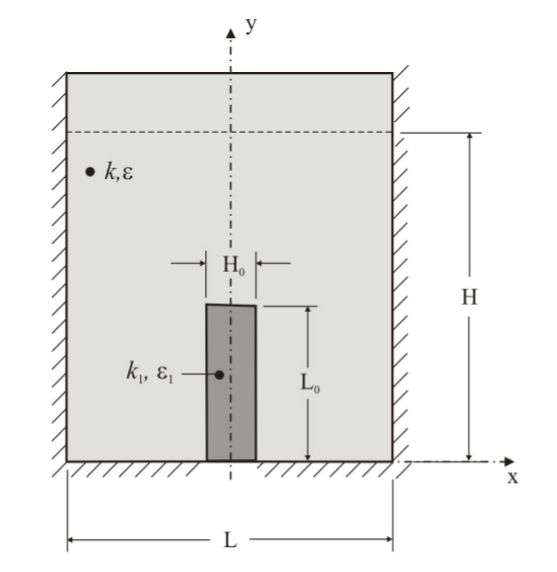
\includegraphics[width=.7\linewidth]{img/dominio}
\caption{Ilustração do domínio computacional}
\label{figExemplo}
%\vskip -6pt
\end{figure}
	
	

\subsection{Formatação das tabelas}

As tabelas devem ser inseridas de forma centralizada e com o título acima desta.

A numeração de ser por capítulos.

Estas devem sempre ser citadas no texto antes de sua aparição. A forma de citação deve ser

... os dados são mostrados na Tab. \ref{tabExemplo} ... quando da citação no meio do texto e na forma 

“... A Tabela \ref{tabExemplo} traz ...” quando de citações no início do texto.

\subsubsection{Exemplo de utilização de tabela}

A Tabela \ref{tabExemplo} traz um resumo do teste de independência de malha.

\begin{table}[h!]
\begin{center}
	\caption{Teste de independência de malha}
	\begin{tabular}{c|c|c|c} \hline
		\textbf{Malha} & \textbf{No de volumes} & \textbf{\textit{Nu}} & \textbf{Desvio} \\ \hline
		M1 & 9347 		& 6,030	 & 6,55\% \\ 
		M2 & 46821 		& 5,635	 & 1,55\% \\
		M3 & 225507		& 5,547	 & 0,196\% \\
		M4 & 495191		& 5,536	 & ------ \\ \hline
	\end{tabular}
	\label{tabExemplo}
\end{center}
\end{table}

	
\subsection{Citações e referências}
% PODE SER UTILIZADO CITAÇÃO VIA BIBTEX USANDO APALIKE
% OU COPIAR O .bbl NO .tex E DEIXAR TUDO EM UM UNICO ARQUIVO.

Podem ser citados trabalhos publicados em artigos de revista como Hirt; Nichols (1981), em livro do tipo \citep{Lamport:LaTeX}, em anais de congressos como \citet{braams:babel}, dissertações Gomes (2010), teses Amorim Júnior (2007) e manuais ESI Group (2014) .

Devem ser evitadas citações de sites de internet.

O formato para as citações e referências deve seguir a norma ABNT.



%--------------------------------------------------------------------------------------------
% REFERENCIAS
\section{REFERÊNCIAS}

\begingroup
\renewcommand{\section}[2]{}%
\begin{thebibliography}{1}

\bibitem[Braams, 1991]{braams:babel}
Braams, J., \newblock {\em Babel, a multilingual style-option system for use with latex's standard document styles}. \newblock TUGboat, 12(2):291--301, 1991.

\bibitem[Lamport, 1986]{Lamport:LaTeX}
Lamport, L. \newblock {\bf LaTeX User's Guide and Document Reference Manual}. \newblock Addison-Wesley Publishing Company, Reading, Massachusetts, 1986.

\end{thebibliography}
\endgroup


%--------------------------------------------------------------------------------------------
%\addtocontents{toc}{\protect\setcounter{tocdepth}{1}}
\section{ANEXOS}

Os Anexos apresentam textos e documentos não elaborados pelo autor, mas que servem para fundamentar, comprovar ou ilustrar as ideias do trabalho, sem prejuízo da apresentação nem do desenvolvimento do texto.

Todos os anexos devem ser citados no texto.


\subsection{Anexo 1 - Catálogo de parafusos, porcas e arruelas de Ciser}
\begin{figure}[h]
\centering
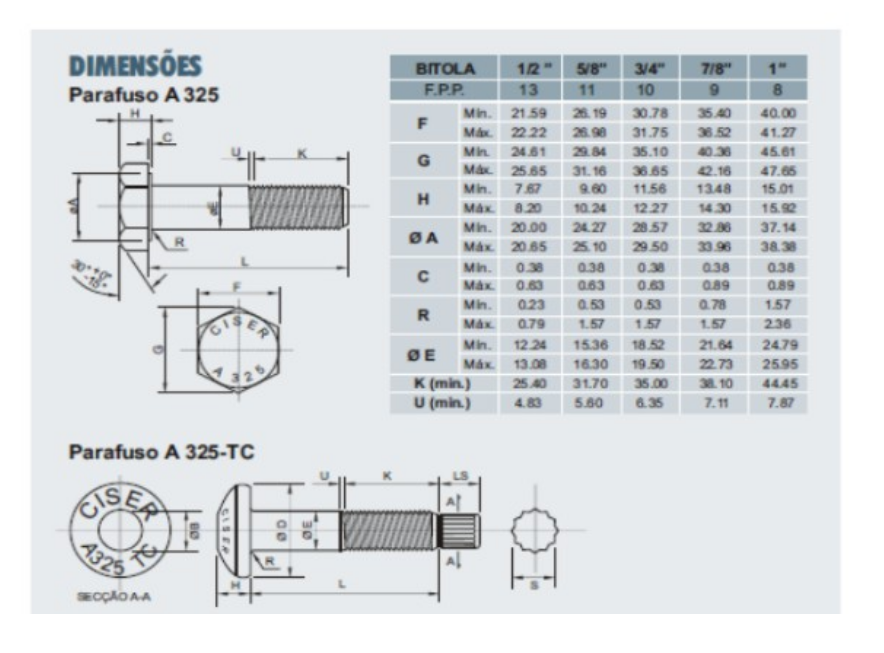
\includegraphics[width=1\linewidth]{img/catalogo}
%\vskip -6pt
\end{figure}

\section{APÊNDICES}

Apêndices são elementos opcionais onde aparecem textos ou documentos elaborados pelo próprio autor, a fim de complementar sua argumentação, sem prejuízo da apresentação e
desenvolvimento normal do texto.


Todos os apêndices devem ser citados no texto.


\subsection{Apêndice 1 - Código utilizado para aplicação das condições de contorno}

\begin{figure}[h]
\centering
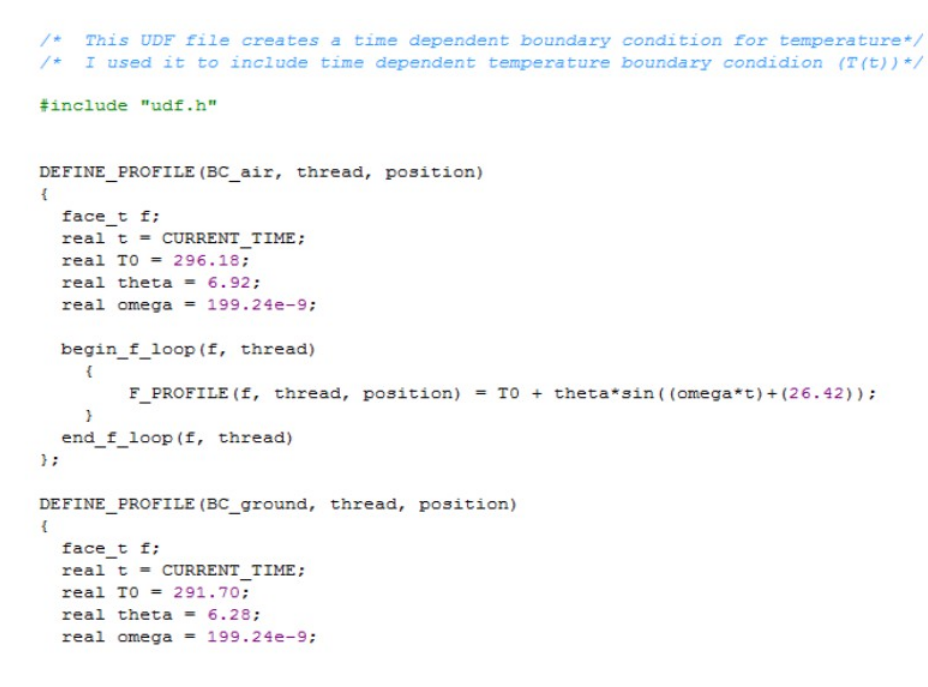
\includegraphics[width=1\linewidth]{img/codigo}
%\vskip -6pt
\end{figure}

\end{document}